\documentclass[a4paper,12pt]{article}

\usepackage[utf8]{inputenc}
\usepackage[T1]{fontenc}
\usepackage[brazilian]{babel}

\usepackage{graphicx}

\usepackage{geometry}

\usepackage{caption}

\geometry{margin=1in}

\title{Modelo Relacional UML da Aplicação CAMAAR}

\author{Weldo Gonçalves da Silva Junior -- 222014133 \\
Daniel Dezan Baby -- 232046097 \\
Leonardo Tome Sampaio -- 222005448 \\
Luis Eduardo Curi Serra -- 251033574 \\
Tarsila Marques de Oliveira Alves -- 242012029}

\date{}

\begin{document}

\maketitle

\section*{Introdução}

A aplicação \textbf{CAMAAR} (Sistema para avaliação de atividades acadêmicas remotas do CIC) é um sistema desenvolvido em \textit{Ruby on Rails} para a avaliação das turmas do CIC. O administrador importa do SIGAA as turmas, matérias e participantes, monta \textit{templates} de formulário e envia formulários de avaliação para as turmas escolhidas. Discentes e docentes respondem a esses formulários, e o administrador baixa os resultados em CSV. Este relatório apresenta o modelo relacional UML da aplicação, descrevendo suas principais entidades, atributos e relacionamentos.

O modelo foi construído a partir das histórias de usuário das \textit{issues} \#98 a \#113 do repositório EngSwCIC/CAMAAR e dos arquivos \texttt{classes.json} e \texttt{class\_members.json}, que mostram o formato dos dados exportados pelo SIGAA. Os nomes das entidades e dos atributos estão em inglês, seguindo as convenções do \textit{Rails}, com a tradução entre parênteses.

\section*{Entidades Principais}

\subsection*{1. User (Usuário)}

\begin{itemize}

    \item \textbf{id}: Identificador único (chave primária).

    \item \textbf{name}: Nome completo do usuário.

    \item \textbf{email}: E-mail do usuário (único); usado no login e no envio dos links de definição e de redefinição de senha.

    \item \textbf{registration}: Matrícula do discente ou, no caso do docente, o usuário do SIGAA (único); também pode ser usado no login (\textit{issue} \#104).

    \item \textbf{password\_digest}: Senha criptografada. Fica nula até o usuário definir a senha pelo link recebido por e-mail, e só então o cadastro é efetivado (\textit{issues} \#100 e \#105).

    \item \textbf{admin}: Indica se o usuário é administrador; nesse caso, o menu lateral mostra a opção de gerenciamento (\textit{issue} \#104).

    \item \textbf{course}: Curso do discente (e.g., CIÊNCIA DA COMPUTAÇÃO/CIC).

    \item \textbf{education\_level}: Formação do usuário (e.g., graduando, DOUTORADO).

    \item \textbf{token\_digest}: Versão criptografada do \textit{token} enviado no link de definição ou de redefinição de senha (\textit{issues} \#105 e \#107).

    \item \textbf{token\_expires\_at}: Data e hora em que o \textit{token} deixa de valer (48 horas após o envio).

    \item \textbf{department\_id}: Chave estrangeira associada ao departamento (opcional). Vem do SIGAA para os docentes e é informada no cadastro dos administradores (\textit{issue} \#106).

\end{itemize}

Relacionamento: Um usuário pertence a nenhum ou a um departamento, participa de nenhuma ou várias turmas e envia nenhuma ou várias respostas. Um administrador cria nenhum ou vários templates e formulários.

\subsection*{2. Department (Departamento)}

\begin{itemize}

    \item \textbf{id}: Identificador único (chave primária).

    \item \textbf{name}: Nome do departamento como vem do SIGAA (e.g., DEPTO CIÊNCIAS DA COMPUTAÇÃO); único.

\end{itemize}

Relacionamento: Um departamento tem nenhum ou vários usuários e oferece nenhuma ou várias matérias.

\subsection*{3. Subject (Matéria)}

\begin{itemize}

    \item \textbf{id}: Identificador único (chave primária).

    \item \textbf{code}: Código da matéria no SIGAA (e.g., CIC0097); único.

    \item \textbf{name}: Nome da matéria (e.g., BANCOS DE DADOS).

    \item \textbf{department\_id}: Chave estrangeira associada ao departamento que oferece a matéria (opcional). Como o \texttt{classes.json} não traz o departamento, ele é preenchido na importação com o departamento do docente da turma, que vem no \texttt{class\_members.json}.

\end{itemize}

Relacionamento: Uma matéria é oferecida por nenhum ou um departamento e possui nenhuma ou várias turmas.

\subsection*{4. SchoolClass (Turma)}

\begin{itemize}

    \item \textbf{id}: Identificador único (chave primária).

    \item \textbf{subject\_id}: Chave estrangeira associada à matéria.

    \item \textbf{code}: Código da turma (e.g., TA).

    \item \textbf{semester}: Semestre letivo (e.g., 2021.2). O semestre atual é o mais recente importado.

    \item \textbf{schedule}: Horário no formato do SIGAA (e.g., 35T45).

\end{itemize}

Relacionamento: Cada turma pertence a uma matéria, tem nenhum ou vários participantes e recebe nenhum ou vários formulários. A combinação (\texttt{subject\_id}, \texttt{code}, \texttt{semester}) é única, o que permite importar e atualizar os dados do SIGAA sem duplicar turmas (\textit{issues} \#98 e \#108). O nome \texttt{SchoolClass} evita o conflito com a classe \texttt{Class} do Ruby.

\subsection*{5. Participation (Participação)}

\begin{itemize}

    \item \textbf{id}: Identificador único (chave primária).

    \item \textbf{user\_id}: Chave estrangeira associada ao usuário.

    \item \textbf{school\_class\_id}: Chave estrangeira associada à turma.

    \item \textbf{role}: Papel do usuário na turma: \texttt{student} (discente) ou \texttt{teacher} (docente). Na importação, os valores \texttt{dicente} e \texttt{docente} do campo \texttt{ocupacao} do SIGAA são convertidos para esses dois.

\end{itemize}

Relacionamento: Cada participação liga um usuário a uma turma. É a entidade associativa da relação muitos-para-muitos entre \texttt{User} e \texttt{SchoolClass}, preenchida a partir do \texttt{class\_members.json}; o par (\texttt{user\_id}, \texttt{school\_class\_id}) é único.

\subsection*{6. FormTemplate (Template de Formulário)}

\begin{itemize}

    \item \textbf{id}: Identificador único (chave primária).

    \item \textbf{title}: Nome do template (até 100 caracteres, sem repetir entre os templates do mesmo administrador).

    \item \textbf{creator\_id}: Chave estrangeira associada ao administrador que criou o template.

    \item \textbf{created\_at}: Data de criação.

\end{itemize}

Relacionamento: Cada template é criado por um administrador, contém nenhuma ou várias questões e dá origem a nenhum ou vários formulários (\textit{issues} \#102 e \#111). Um template sem questões pode ser salvo, mas não pode gerar formulário.

\subsection*{7. Question (Questão)}

\begin{itemize}

    \item \textbf{id}: Identificador único (chave primária).

    \item \textbf{form\_template\_id}: Chave estrangeira associada ao template (preenchida nas questões do template).

    \item \textbf{form\_id}: Chave estrangeira associada ao formulário (preenchida nas cópias feitas quando o formulário é criado).

    \item \textbf{statement}: Texto da pergunta.

    \item \textbf{question\_type}: Tipo da questão: \texttt{radio} (escolha de uma opção) ou \texttt{text} (resposta livre), os dois tipos do protótipo. O nome evita a coluna \texttt{type}, reservada pelo \textit{Rails}.

    \item \textbf{position}: Posição da questão no template ou no formulário.

    \item \textbf{required}: Indica se a resposta é obrigatória.

\end{itemize}

Relacionamento: Cada questão pertence a um template ou a um formulário (exatamente uma das duas chaves é preenchida), tem nenhuma ou várias opções e é respondida em nenhum ou vários itens de resposta.

\subsection*{8. Option (Opção)}

\begin{itemize}

    \item \textbf{id}: Identificador único (chave primária).

    \item \textbf{question\_id}: Chave estrangeira associada à questão.

    \item \textbf{text}: Texto da alternativa.

    \item \textbf{position}: Posição da alternativa na questão.

\end{itemize}

Relacionamento: Cada opção pertence a uma questão do tipo \texttt{radio}, que precisa de pelo menos duas opções, e pode ser escolhida em nenhum ou vários itens de resposta.

\subsection*{9. Form (Formulário)}

\begin{itemize}

    \item \textbf{id}: Identificador único (chave primária).

    \item \textbf{form\_template\_id}: Chave estrangeira associada ao template de origem (opcional; fica nula se o template for excluído).

    \item \textbf{school\_class\_id}: Chave estrangeira associada à turma avaliada.

    \item \textbf{creator\_id}: Chave estrangeira associada ao administrador que criou o formulário.

    \item \textbf{title}: Título copiado do template, para o formulário continuar identificado mesmo que o template seja excluído.

    \item \textbf{target\_audience}: Público-alvo do formulário: \texttt{students} (discentes, o padrão) ou \texttt{teachers} (docentes) (\textit{issue} \#113).

    \item \textbf{created\_at}: Data de criação.

\end{itemize}

Relacionamento: Cada formulário avalia uma turma, é criado por um administrador e tem origem em nenhum ou um template. Ele contém uma ou várias questões, que são cópias das questões do template, e recebe nenhuma ou várias respostas. O administrador escolhe o template e as turmas, e o sistema cria um formulário por turma (\textit{issue} \#103); a lista desses formulários é a base da visualização dos resultados (\textit{issue} \#110). Como as questões são copiadas, editar ou excluir o template depois não altera o formulário (\textit{issue} \#112).

\subsection*{10. Submission (Resposta)}

\begin{itemize}

    \item \textbf{id}: Identificador único (chave primária).

    \item \textbf{form\_id}: Chave estrangeira associada ao formulário respondido.

    \item \textbf{user\_id}: Chave estrangeira associada ao participante que respondeu.

    \item \textbf{submitted\_at}: Data e hora do envio.

\end{itemize}

Relacionamento: Cada resposta pertence a um formulário e a um participante e é composta por um ou vários itens (\textit{issue} \#99). O par (\texttt{form\_id}, \texttt{user\_id}) é único, então cada participante responde uma única vez a cada formulário. Os formulários pendentes de um participante (\textit{issue} \#109) são os das suas turmas, com público-alvo igual ao seu papel na turma, que ainda não têm resposta dele.

\subsection*{11. Answer (Item de Resposta)}

\begin{itemize}

    \item \textbf{id}: Identificador único (chave primária).

    \item \textbf{submission\_id}: Chave estrangeira associada à resposta.

    \item \textbf{question\_id}: Chave estrangeira associada à questão do formulário que foi respondida.

    \item \textbf{option\_id}: Chave estrangeira associada à opção escolhida (opcional; só em questões do tipo \texttt{radio}).

    \item \textbf{text\_value}: Texto digitado nas questões do tipo \texttt{text} (até 1000 caracteres).

\end{itemize}

Relacionamento: Cada item pertence a uma resposta e a uma questão e, nas questões do tipo \texttt{radio}, a uma opção. Uma resposta tem no máximo um item por questão. O relatório em CSV (\textit{issue} \#101) é gerado sob demanda a partir desses itens, por isso não é uma entidade do modelo.

\clearpage

\section*{Modelo Relacional UML}

Abaixo está o modelo relacional UML que descreve a estrutura de dados da aplicação \textbf{CAMAAR}:

\begin{figure}[h!]

    \centering

    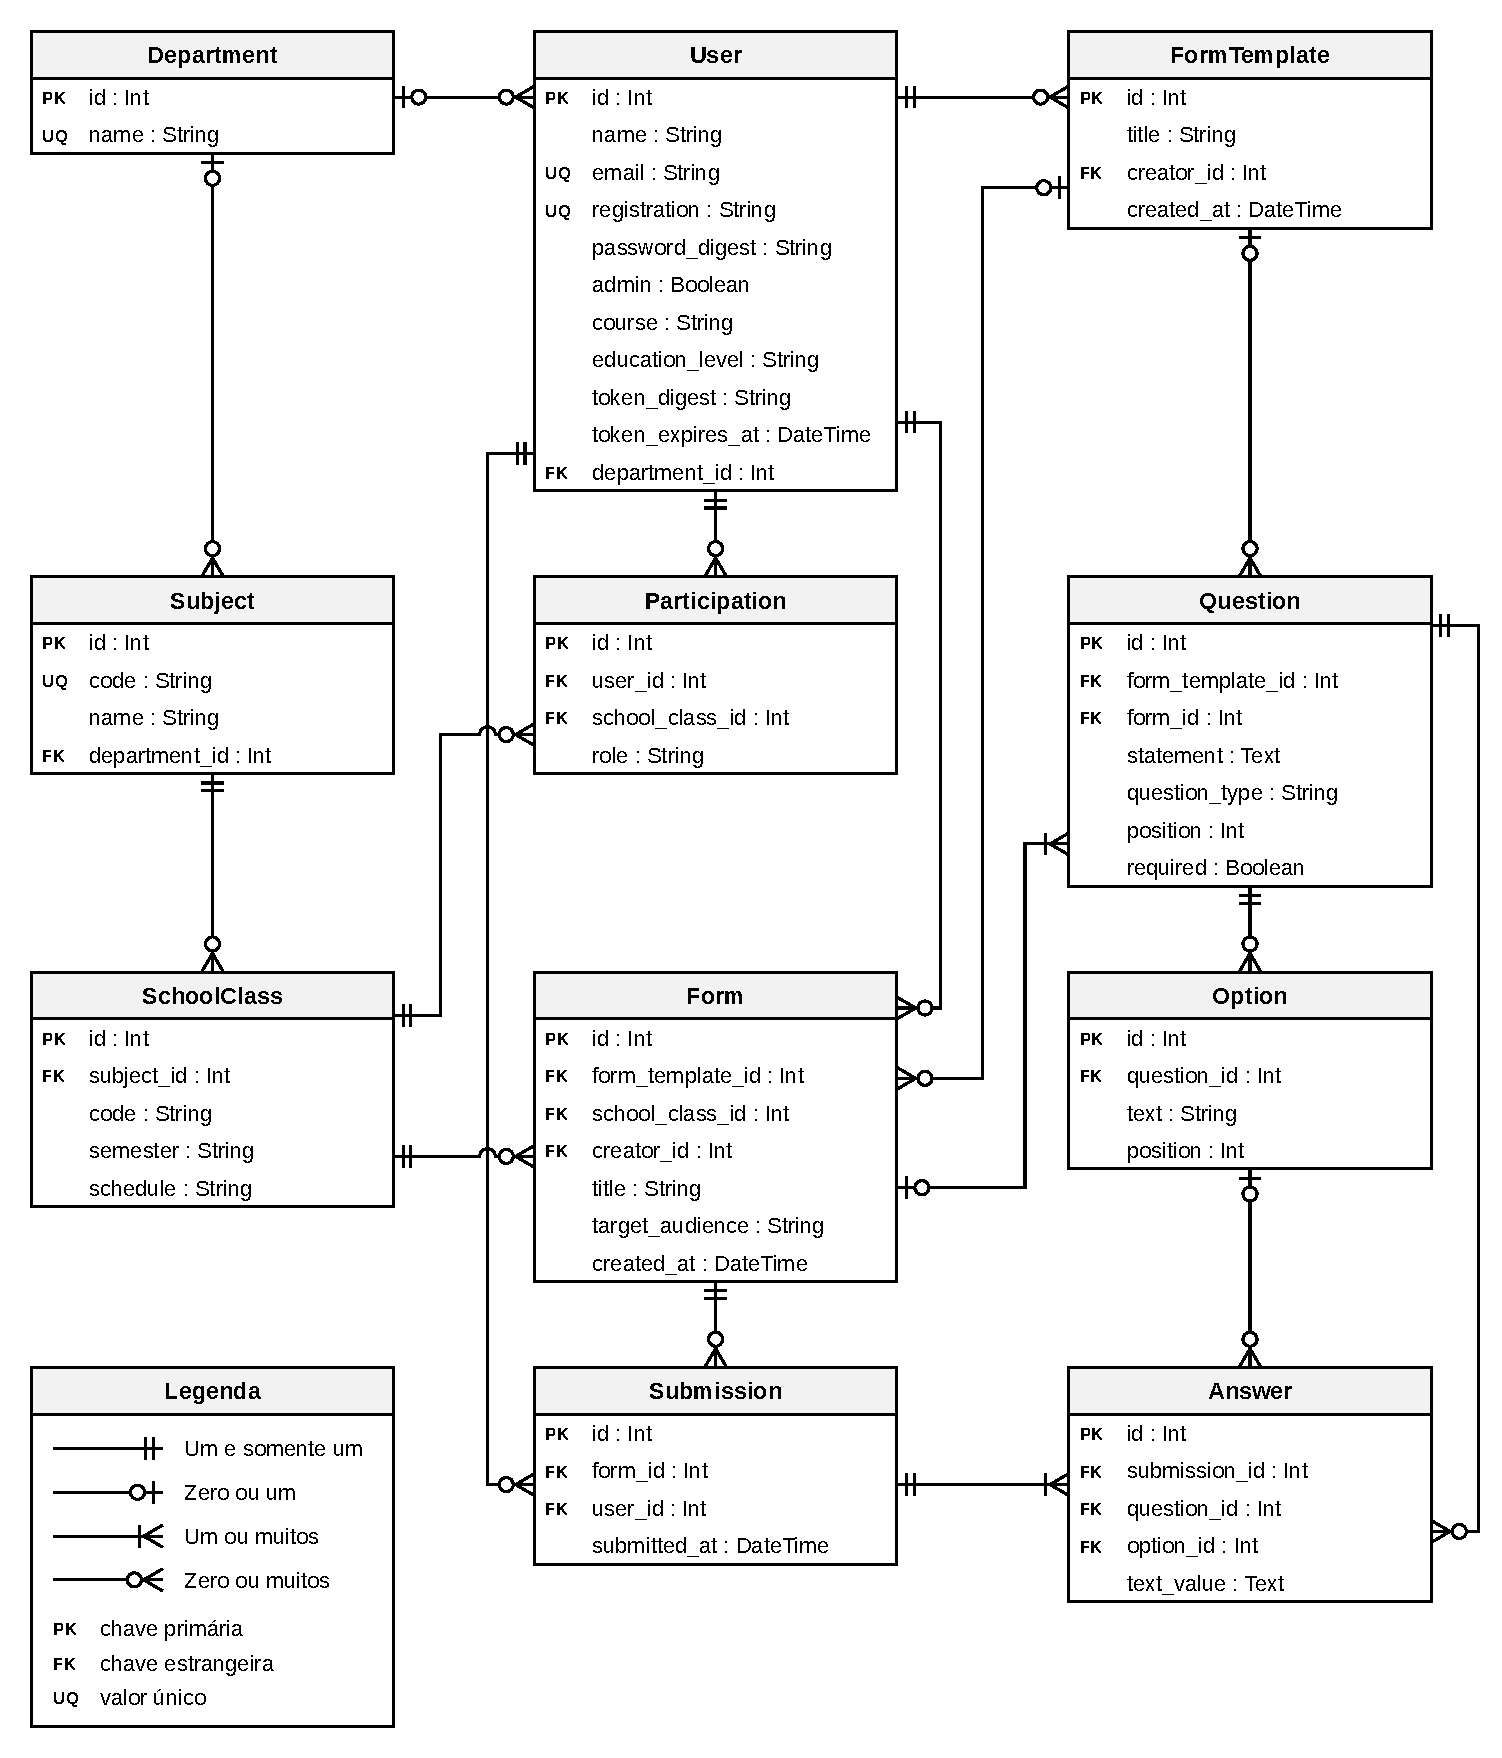
\includegraphics[width=\textwidth]{er-camaar-v2.pdf}

    \caption{Modelo Relacional UML da aplicação CAMAAR.}

    \label{fig:uml}

\end{figure}

\section*{Considerações Finais}

O modelo apresentado atende às histórias de usuário \#98 a \#113: importação e atualização dos dados do SIGAA, cadastro por e-mail, login, definição e redefinição de senha, criação e gestão de templates, envio de formulários por turma e por público-alvo, resposta aos formulários e geração do relatório em CSV. As principais decisões de modelagem foram: (i) copiar as questões e as opções do template para cada formulário no momento do envio, para que editar ou excluir um template não altere formulários e respostas que já existem (\textit{issue} \#112); (ii) guardar o papel de discente ou docente na participação, e não no usuário, que só indica se é administrador; (iii) usar chaves naturais únicas (código da matéria; matéria, turma e semestre; matrícula) para que importar os mesmos dados de novo não crie registros duplicados (\textit{issues} \#98 e \#108); e (iv) manter a avaliação anônima no relatório: a resposta guarda o participante só para impedir respostas repetidas e para listar os formulários pendentes, e o CSV não exporta essa informação.

As entidades \texttt{Department} e \texttt{Participation} deixam o modelo preparado para a funcionalidade bônus de gerenciamento por departamento (\textit{issue} \#106), e o modelo pode ser expandido, por exemplo, com prazos de resposta para os formulários ou com novos tipos de questão.

\end{document}
